\documentclass[12pt,letter]{article}
\usepackage{mathptmx} % added for time new roman font
\usepackage[left=1in,right=1in,top=1in,bottom=1in]{geometry}
\usepackage[latin1]{inputenc}
\usepackage{amsmath}

% defines all example enviorment
\usepackage[framemethod=tikz]{mdframed} % added for the box around examples
\newtheorem{ex}{Example}
\numberwithin{ex}{section} % allows for the use of example numbers that lign up with the section numbers
\newenvironment{example}{\begin{mdframed}[middlelinewidth=0.5mm]\begin{ex}\normalfont}{\end{ex}\end{mdframed}}

% defines all review enviorment
\usepackage[framemethod=tikz]{mdframed} % added for the box around examples
\newtheorem{re}{Review}
\numberwithin{re}{section} % allows for the use of example numbers that lign up with the section numbers
\newenvironment{review}{\begin{mdframed}[middlelinewidth=2mm,roundcorner=20pt]\begin{re}\normalfont}{\end{re}\end{mdframed}}

% defines the quotation enviorment 
\usepackage{xcolor}
\newcommand{\quotebox}[2]{\begin{center}\fcolorbox{white}{blue!15!gray!15}{\begin{minipage}{0.9\linewidth}\vspace{10pt}\center\begin{minipage}{0.8\linewidth}{\space\Huge``}{#1}{\Huge''}{\break\null\hfill} {\small #2}  \end{minipage}\medbreak\end{minipage}}\end{center}}

% defines the definition enviorment 
\newcommand{\definitionbox}[2]{\begin{center}\fcolorbox{white}{blue!15!gray!15}{\begin{minipage}{0.9\linewidth}\vspace{10pt}\center\begin{minipage}{0.8\linewidth} {{\textbf{Definition} - }{#1}: {#2}}\end{minipage}\medbreak\end{minipage}}\end{center}}

\usepackage{amsfonts}
\usepackage{amssymb}
\usepackage{graphicx}
\usepackage{float}
\usepackage{booktabs}
%\usepackage{parskip} % remove all the paragraph indents
\usepackage[textsize=tiny]{todonotes}


\usepackage{setspace}
\usepackage[colorlinks=true]{hyperref}
\usepackage{textcomp} 
\usepackage{multicol} 

% added for MATLAB code
\usepackage[framed]{matlab-prettifier}
\let\ph\mlplaceholder % shorter macro
\lstMakeShortInline"

\lstset{
  style              = Matlab-editor,
  basicstyle         = \mlttfamily,
  escapechar         = ",
  mlshowsectionrules = true,
}



\usepackage{color} % color added for editing
\newcommand{\bl}[1]{\textcolor[rgb]{0.00,0.00,1.00}{#1}}
\newcommand{\gr}[1]{\textcolor[rgb]{0.00,0.50,0.00}{#1}}
\newcommand{\rd}[1]{\textcolor[rgb]{0.75,0.00,0.00}{#1}}
\newcommand{\tl}[1]{\textcolor[rgb]{0,0.6,0.60}{#1}}



%%%%%%%		define the symbols for positive directions		%%%%%%
\makeatletter													%%	
																%%					
\newcommand*\curveplus{% positive counterclockwise				%%
  \mathbin{\rotatebox[origin=c]{90}{$\m@th\curvearrowleft$}+}}	%%
																%%
\newcommand*\rightplus{% positive right							%%
  \mathpalette\@rightplus\relax}								%%
\newcommand*\@rightplus[1]{%									%%
  \mathbin{\vcenter{\hbox{$\m@th\overset{#1+}{\to}$}}}}			%%
																%%	
\newcommand*\upplus{% positive up								%%
  \mathbin{+\mathord\uparrow}}									%%
																%%			
\newcommand*\downplus{% positive down							%%		
  \mathbin{+\mathord\downarrow}}								%%
  																%%		
\newcommand*\downrightplus{% positive down and right			%%	
  \mathbin{+ \rotatebox[origin=c]{-30}{$\m@th\rightarrow$}}}	%%
\makeatother 													%%	
%%%%%%%%%%%%%%%%%%%%%%%%%%%%%%%%%%%%%%%%%%%%%%%%%%%%%%%%%%%%%%%%%%


\usepackage{mathtools}          %loads amsmath as well added for the piece wise function
\DeclarePairedDelimiter\Floor\lfloor\rfloor
\DeclarePairedDelimiter\Ceil\lceil\rceil

 
\newcounter{NumberInTable}
\newcommand{\LTNUM}{\stepcounter{NumberInTable}{(\theNumberInTable)}}

\newcommand{\Laplace}[1]{\ensuremath{\mathcal{L}{\left[#1\right]}}}
\newcommand{\InvLap}[1]{\ensuremath{\mathcal{L}^{-1}{\left[#1\right]}}}
\renewcommand{\textuparrow}{$\uparrow$}


\begin{document}
	
	% set the section number, along with figure and equation numbers
	\setcounter{section}{8}	
	\setcounter{figure}{0}   
	\renewcommand\thefigure{\thesection.\arabic{figure}}
	\setcounter{equation}{0}   
	\renewcommand\theequation{\thesection.\arabic{equation}}

	\section{Experimental Vibrations}
	
Experimental vibration testing requires the practitioner to understand the basics of testing hardware and digital signal processing.

\subsection{Modal Analysis}


\begin{figure}[H]
    \centering
    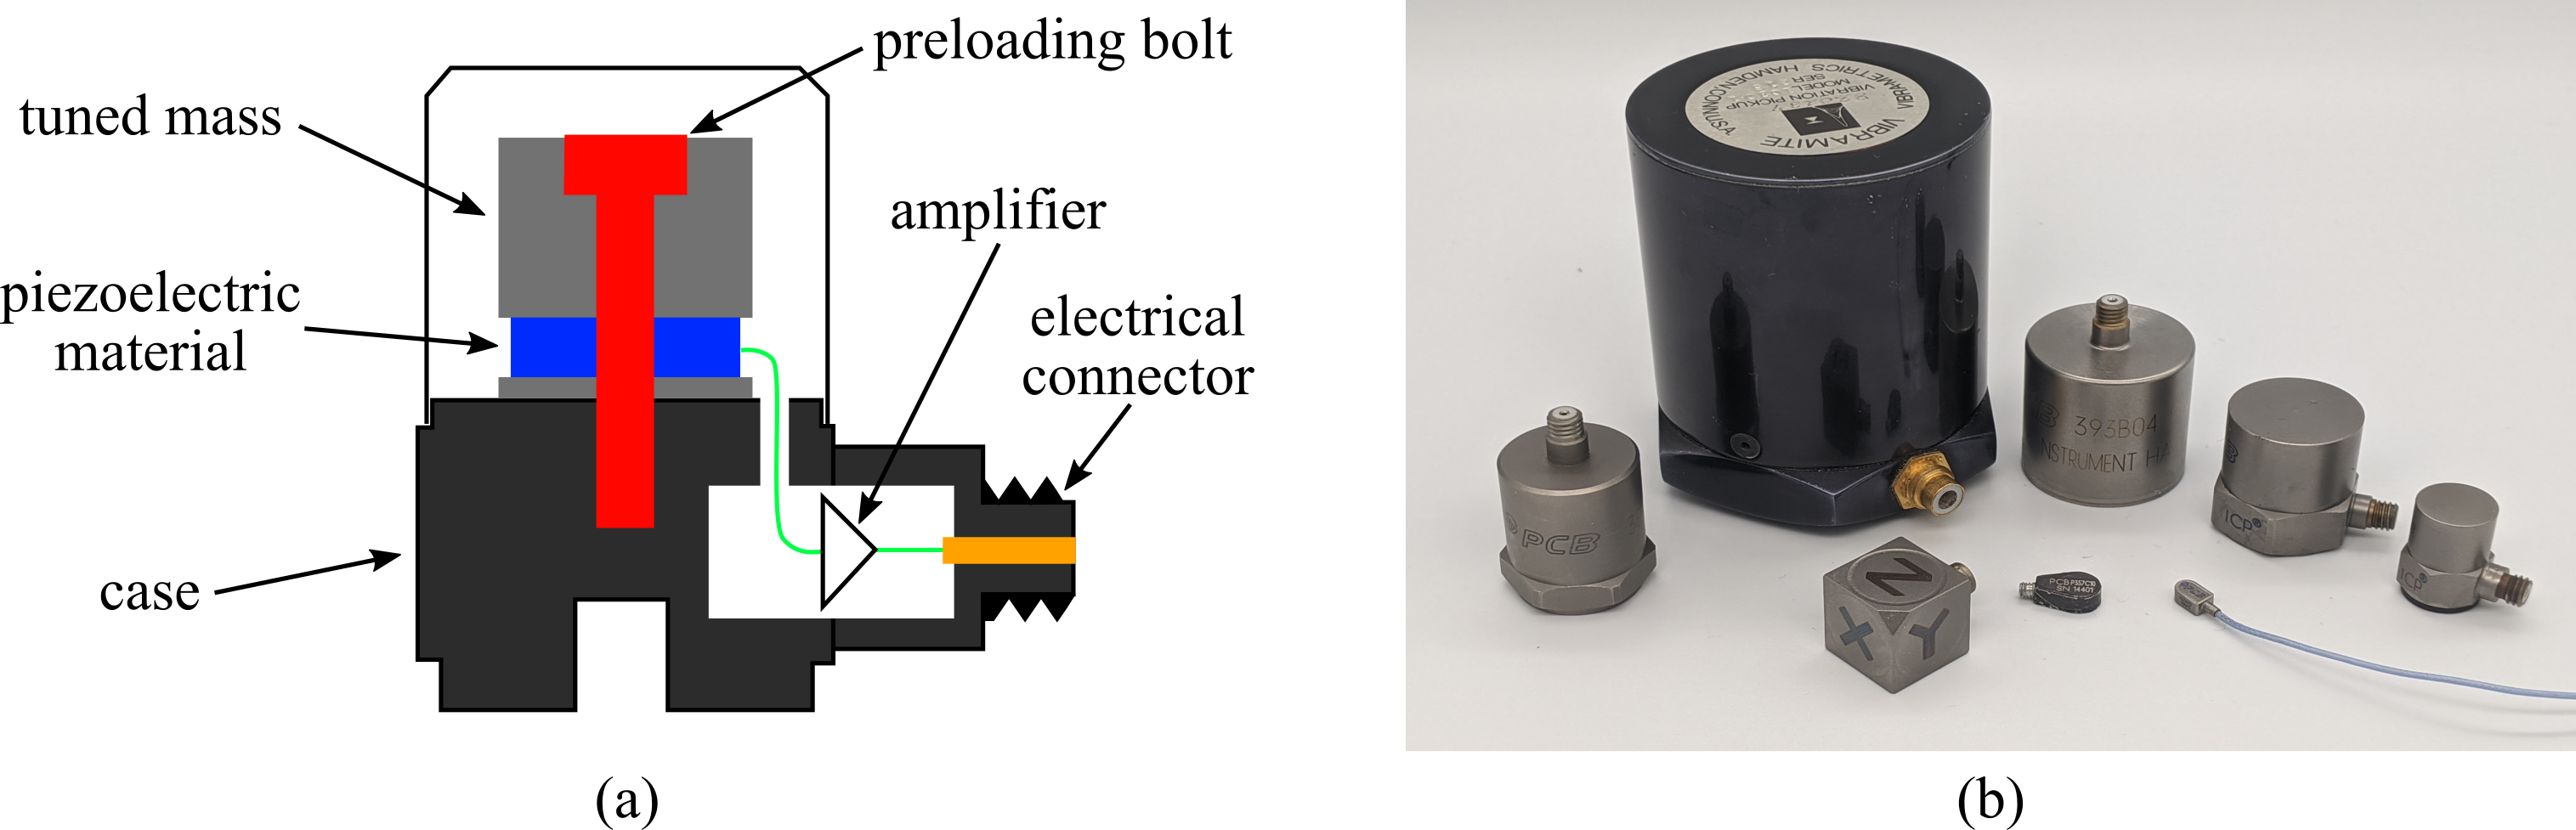
\includegraphics[]{figures/accelerometers.png}
    \caption{Integrated Electronics Piezo-Electric (IEPE) accelerometers, showing: (a) the cross section of a typical IEPE) accelerometer with key components annotated, and; (b) selection of IEPE accelerometers for various applications.}
    \label{fig:accelerometers}
\end{figure} 

\begin{itemize}
\item window
\item segment length
\item overlap
\end{itemize}

\maketitle
\section{METHODOLOGY}
%\begin{abstract}
To experimentally determine the vertical mode shapes for simple beam structures the following process is applicable. 

First, accelerometers are evenly spaced and attached to the beam along its length as shown in Figure~\ref{fig:PhysicalTestBed}. This provides acceleration data for various locations on the beam, for the beam in Figure~\ref{fig:PhysicalTestBed} only 4 accelerometers are used with a DAQ system and data collection software to determine the first few vertical modes. However, to determine higher vertical modes more accelerometers will be needed to measure the increasing number of nodes and anti-nodes.    

%Take a new picture for Figure 1 that has actual acc. on it 
\begin{figure}[b]
	\centering 
	\includegraphics*[width= 1\linewidth]{figures/Testbed/PhysicalTestbed.png}
	\vspace{0.1cm}
	\caption{Physical testbed that consists of a cantilever beam with movable support on the right-hand-side and a shaker to represent the structure of interest.}
	\label{fig:PhysicalTestBed}
\end{figure}


Second, the test beam is excited with a frequency sweep (chirp signal) using a function generator to create the the input signal, power amplifier to gradually amplify the input signal, and a shaker to apply the frequency sweep to the beam. This provides every frequency as an input that the beam uniquely reacts to. Continuing, while the frequency sweep is active, acceleration data is collected at each accelerometer location for the entire sweep duration and is used to determine each modal frequency of beam by taking an FFT.


Third, after the frequency sweep and acceleration data collection is completed, a Fast Fourier Transform (FFT) Figure~\ref{fig:FFT}, of the acceleration data is performed to determine the specific modal frequencies. Moreover, the FFT shows the frequencies at which beam deformation occurs, where the lowest frequency that causes deformation is the first mode, the next frequency is the second mode and so on. With the FFTs completed, each modal frequency is now known and the beam can be excited at each individual modal frequency to determine the specific amplitude of deformation each frequency causes. 


%Insert an FFT plot labeled correctly 
\begin{figure}[t]
	\centering 
	\includegraphics*[width= 1\linewidth]{figures/FFT/FFT.png}
	\vspace{0.1cm}
	\caption{FFT of acceleration data.}
	\label{fig:FFT}
\end{figure}



%Insert an In phase plot labeled correctly 
\begin{figure}[b]
	\centering 
	\includegraphics*[width= 1\linewidth]{figures/InPhase/InPhase.png}
	\vspace{0.1cm}
	\caption{In phase accelerometers.}
	\label{fig:InPhase}
\end{figure}



\newpage
Forth, before specific amplitudes are found nodal locations for each modal frequency need to be determined. Moreover, this is achieved while the beam is excited at a modal frequency, the nodes are found by moving a screw driver along the beam length. This is an easy method since the nodes are locations of zero movement its easy to feel and hear the vibration differences between a node and non-node. Once the nodes are found, the same process is used to find the anti-nodes (locations of maximum displacement). This is also easy since these locations vibrate considerably more than any other location along the beam. Continuing, after each node and anti-node is narrowed to a small location, each accelerometer is moved to each node and anti-node to determine the specific amplitudes. Since the accelerometers only provides an amplitude, there is a need to check whether each anti-node is in or out of phase. Checking the anti-node phase provides the direction (positive or negative)and validates the mode shapes. 





Fifth, to determine the phase of each anti-node a phase graph of each anti-nodes' accelerometer data is preformed. If the anti-nodes are in phase, the graph shows overlapping data, Figure~\ref{fig:InPhase} and if they are out of phase the graph shows a 180 degree difference between both anti-node accelerometer data shown in Figure~\ref{fig:OutofPhase}. Moreover, if the anti-nodes are in phase then both anti-nodes have a positive and negative amplitude at the same time. Henceforth, in phase anti-nodes cant hold opposing directions (where 1 is positive and 1 is negative), while out of phase anti-nodes can but will never hold the same direction at the same time. With anti-node direction and specific amplitude determined, the mode shape for each modal frequency can be precisely plotted. 

%Insert an Out of phase plot labeled correctly 
\begin{figure}[h]
	\centering 
	\includegraphics*[width= 1\linewidth]{figures/OutofPhase/OutofPhase.png}
	\vspace{0.1cm}
	\caption{Out of phase accelerometers.}
	\label{fig:OutofPhase}
\end{figure}



\end{document}














